\documentclass[border=5mm]{standalone}
\usepackage{xcolor}
\usepackage{tikz}
\usetikzlibrary{positioning}
\usetikzlibrary{calc}
\begin{document}

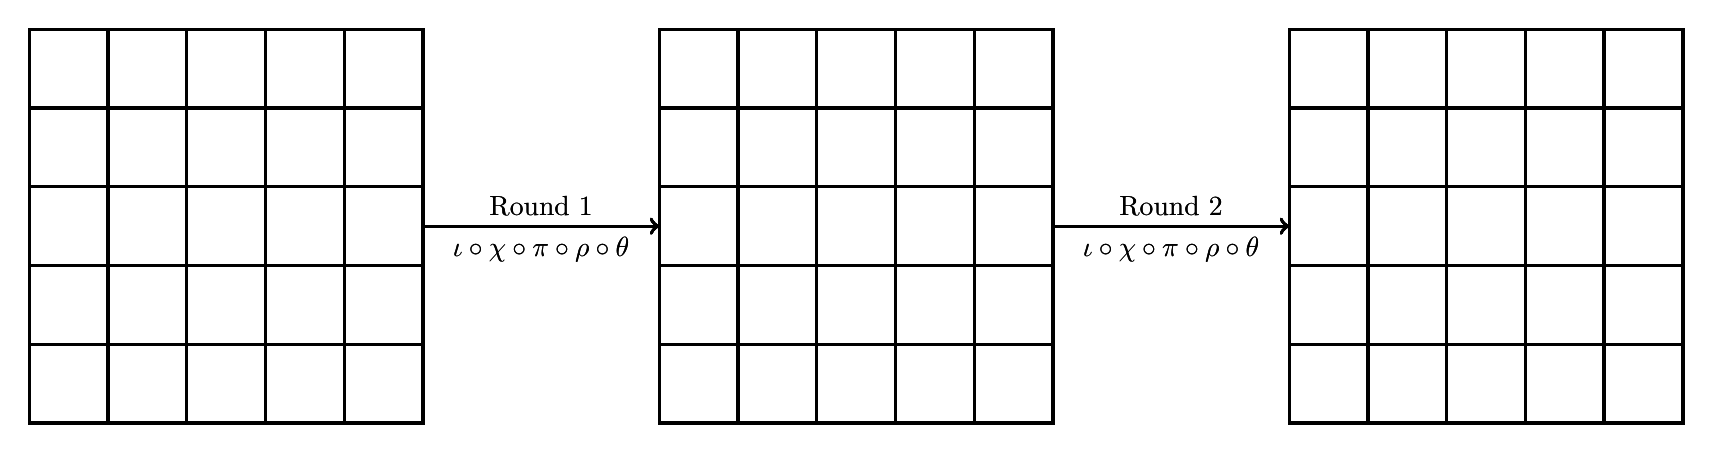
\begin{tikzpicture}
    [%%%%%%%%%%%%%%%%%%%%%%%%%%%%%%
        box/.style={rectangle,draw=black,very thick, minimum size=1cm}
    ]%%%%%%%%%%%%%%%%%%%%%%%%%%%%%%
\definecolor{darkgreen}{rgb}{0.0, 0.7, 0.5}
\foreach \x in {0,1,...,4}{
    \foreach \y in {0,1,...,4}
        \node[box] at (\x,\y){};
}

\foreach \x in {8,...,12}{
    \foreach \y in {0,1,...,4}
        \node[box] at (\x,\y){};
}

\foreach \x in {16,...,20}{
    \foreach \y in {0,1,...,4}
        \node[box] at (\x,\y){};
}

\draw [->,very thick] (4.5,2) -- node [above] {Round $1$} (7.5,2);

\draw [->,very thick] (4.5,2) -- node [below] {$\iota \circ \chi \circ \pi \circ \rho \circ \theta$} (7.5,2);

\draw [->,very thick] (4.5,2) -- node [above] {Round $1$} (7.5,2);

\draw [->,very thick] (4.5,2) -- node [below] {$\iota \circ \chi \circ \pi \circ \rho \circ \theta$} (7.5,2);

\draw [->,very thick] (12.5,2) -- node [above] {Round $2$} (15.5,2);

\draw [->,very thick] (12.5,2) -- node [below] {$\iota \circ \chi \circ \pi \circ \rho \circ \theta$} (15.5,2);

\draw [->,very thick] (12.5,2) -- node [above] {Round $2$} (15.5,2);

\draw [->,very thick] (12.5,2) -- node [below] {$\iota \circ \chi \circ \pi \circ \rho \circ \theta$} (15.5,2);

\end{tikzpicture}
\end{document}